%%%%%%%%%%%%%%%%%%%%%%%%%%%%%%%%%%%%%%%%%
%
% (c) 2022 by Jennifer Laaser
%
% This work is licensed under the Creative Commons Attribution-NonCommercial-ShareAlike 4.0 International License. To view a copy of this license, visit http://creativecommons.org/licenses/by-nc-sa/4.0/ or send a letter to Creative Commons, PO Box 1866, Mountain View, CA 94042, USA.
%
% The current source for these materials is accessible on Github: https://github.com/jlaaser/pogil-polymers
%
%%%%%%%%%%%%%%%%%%%%%%%%%%%%%%%%%%%%%%%%%

\renewcommand{\figpath}{content/polymphys/thermal-transitions/crystals/figs}
\renewcommand{\labelbase}{crystals}

\begin{activity}{Polymer Crystals}

\begin{instructornotes}
	This activity introduces students to concepts related to crystallization of polymeric materials.
	
	After completing this activity, students will be able to:
	\begin{enumerate}
		\item Explain how polymer chains are organized in crystalline and semicrystalline samples, over length scales ranging from 1~\AA\ to 10~$\mu$m
		\item Identify the chemical and structural features of polymers that promote or inhibit crystallization
		\item Quantitatively relate the melting temperature of crystals to their lamellar thicknesses
	\end{enumerate}
	
	\subsection*{Activity summary:}
	\begin{itemize}
		\item \textbf{Activity type:} Learning Cycle
		\item \textbf{Content goals:} See above %Glass Transitions of Polymer Materials
		\item \textbf{Process goals:} %https://pogil.org/uploads/attachments/cj54b5yts006cklx4hh758htf-process-skills-official-pogil-list-2015-original.pdf
			\begin{enumerate}
				\item Interpreting chemical structures and schematics
				\item Interpretation and manipulation of mathematical equations
				\item Linking concepts to derive a key result
				\item Written and oral communication of reasoning
			\end{enumerate}
		\item \textbf{Duration:} 50 minutes, including time for class discussion
		\item \textbf{Instructor preparation required:} none beyond knowledge of relevant content
		\item \textbf{Related textbook chapters:}
			\begin{itemize}
				\item \emph{Polymer Chemistry} (Hiemenz \& Lodge), 2nd ed.: Sections 13.1 and 13.4
				\item \emph{Introduction to Polymers} (Young \& Lovell), 3rd ed.: Sections 17.1, 17.4, and 17.8.2
			\end{itemize}
		%\item \textbf{Instructor notes:}
		%	\begin{itemize}
		%		\item \dots
		%	\end{itemize}
	\end{itemize}
	
\end{instructornotes}


\begin{model}[Structures of Polymer Crystals]
	\label{\labelbase:mdl:crystalstructs}
	
	Under the right conditions, some polymers can arrange into highly-ordered, crystalline materials. One common crystalline polymer is poly(ethylene).  A representative structure of crystalline poly(ethylene) is shown below:
	
	\vspace{6pt}
	\centerline{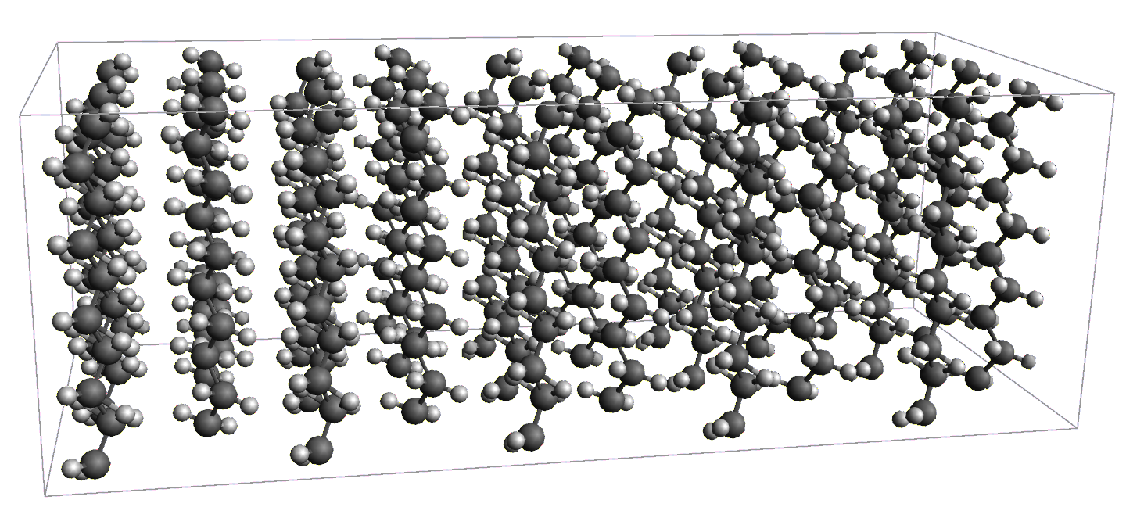
\includegraphics[width=0.6\textwidth]{\figpath/Model1_PE_supercell.pdf}}	
	
	% note for rendering: crystallographic parameters for poly(ethylene) are taken from DOI 10.1039/TF9393500482
	% unit cell dimensions are (7.40, 4.93, 2.534) Angstroms
	% fractional positions of carbon atoms are (0.038, 0.935, 0.250); (0.962, 0.065, 0.750); (0.462, 0.453, 0.750); (0.538, 0.565, 0.250)
	
	A single layer of this crystal, as viewed from the front, appears as follows:
	
	\vspace{6pt}
	\centerline{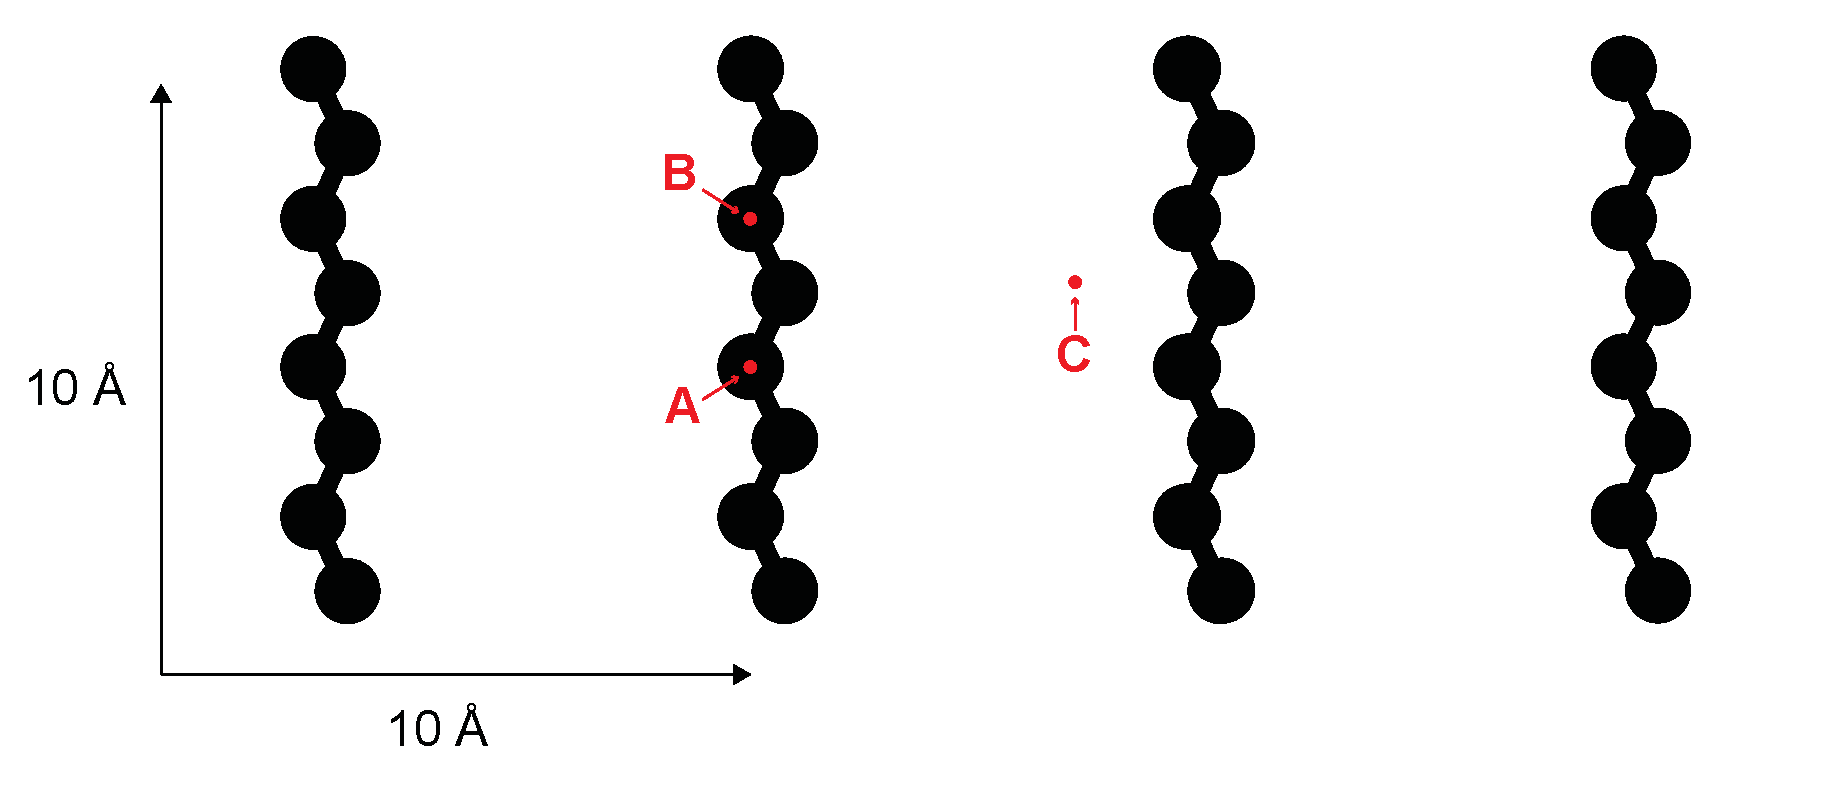
\includegraphics[width=0.6\textwidth]{\figpath/Model1_PE_layer.pdf}}	
	
	For simplicity, only the carbon atoms are shown.
	
\end{model}


\begin{ctqs}

	\question Imagine you are able to shrink yourself down to the atomic scale and walk around on the layer of poly(ethylene) chains shown in the second half of the model.
	
		\begin{enumerate}
			\item If you start at point A and walk to point B, will it look like your environment has changed?  Why or why not?
	
		\begin{solution}[0.75in]{}
			No, it will not look like your environment has changed.  Points A and B are both directly on top of a carbon atom.  Additionally, the ``neighboring'' atoms near point B (both on the same chain and on other chains) are in the same positions relative to point B as the neighboring atoms were to point A.
		\end{solution}
			
			\item If you start at point A and walk to point C, will it look like your environment has changed?  Why or why not?
	
		\begin{solution}[0.75in]{}
			Yes, it will look like your environment has changed.  Point A is directly on top of a carbon atom, while point C is not.
		\end{solution}
			
		\end{enumerate}
		
	\question If you start at point A, what is the minimum distance you would need to walk \textit{in the x direction} to find an environment that looks identical to the one you started in?
	
		\begin{solution}[0.25in]{}
			Approx. 7.5~\AA
		\end{solution}
	
	\question If you start at point A, what is the minimum distance you would need to walk \textit{in the y direction} to find an environment that looks identical to the one you started in?
	
		\begin{solution}[0.25in]{}
			Approx. 2.5~\AA
		\end{solution}
	
	\question On the following image, draw lines indicating each of the minimum distance paths you identified in the previous two questions:

	\begin{solution}[1.25in]{
		\centerline{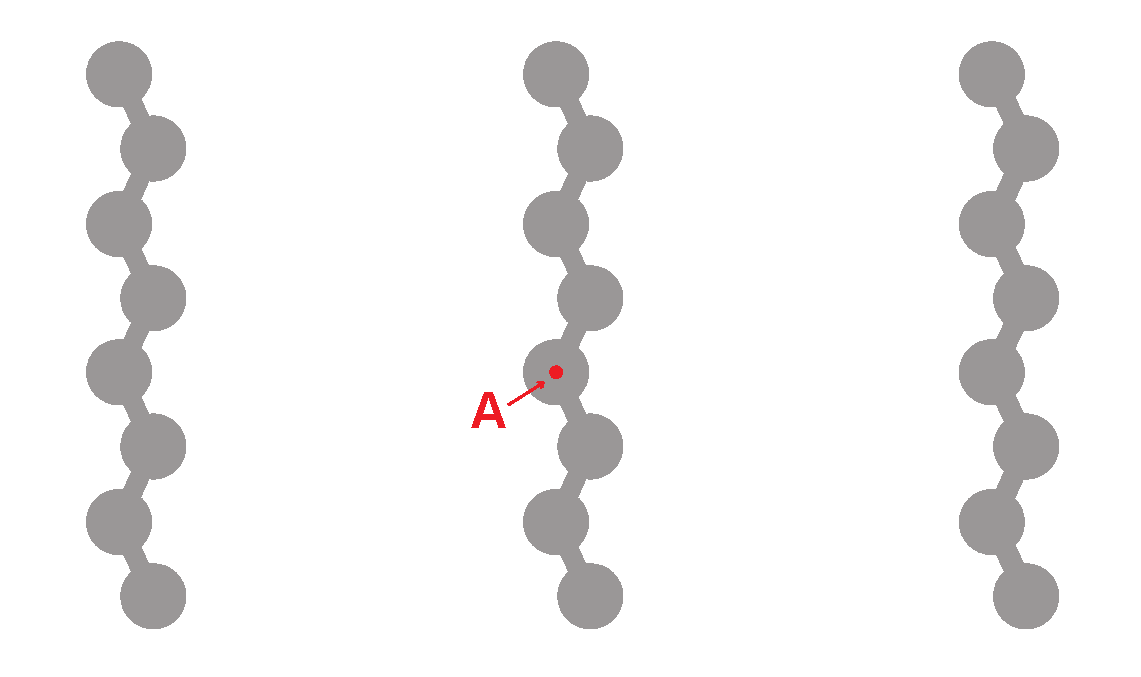
\includegraphics[width=0.35\textwidth]{\figpath/Model1_PE_layer_unitcell_blank.pdf}}	
	}
		\centerline{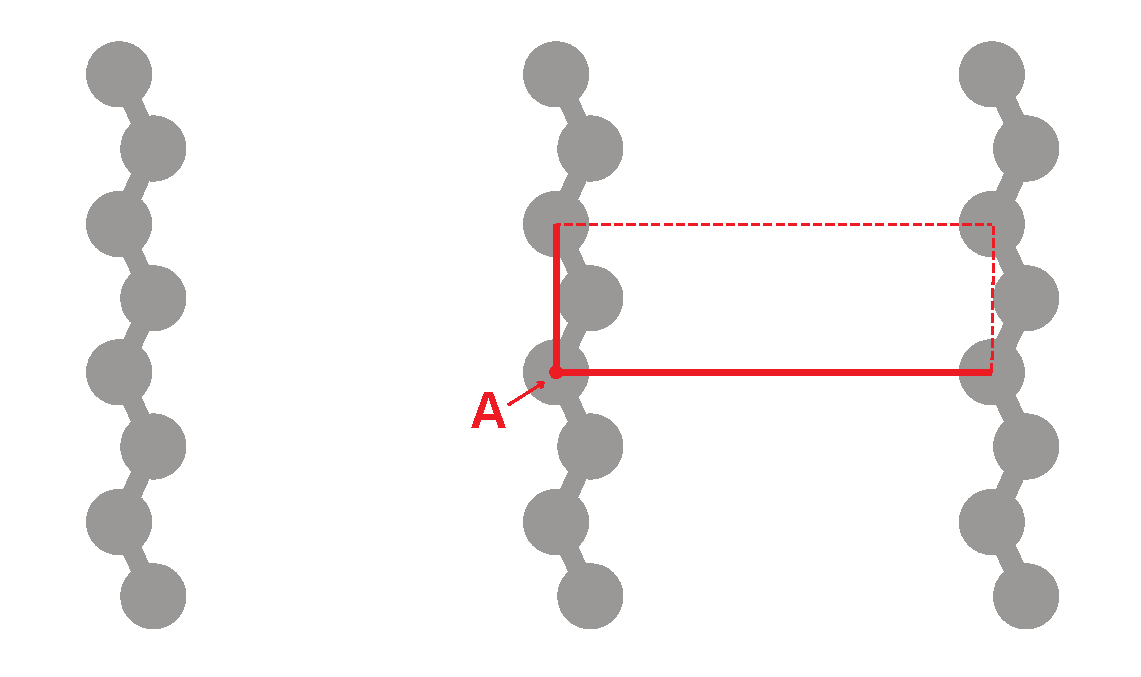
\includegraphics[width=0.35\textwidth]{\figpath/Model1_PE_layer_unitcell_solution.pdf}}
	\end{solution}
	
	\question The two paths you drew in the previous question form two sides of a rectangle.  Draw the other two sides of this rectangle, and explain, in 2-3 complete sentences, why this rectangle can be thought of as the \emph{smallest repeating unit} describing a layer of a poly(ethylene) crystal.
	
		\begin{solution}[1.75in]{}
			If you tile the plane with this rectangle (i.e. use it to make a repeating pattern), then you will get back the original structure.  If we make the rectangle any smaller, then tiling the plane with this rectangle will not result in the same spacing or arrangement of the atoms and polymer chains.  This rectangle is thus the smallest repeating unit that describes this crystal structure.
		\end{solution}
	
\end{ctqs}

\begin{infobox}

	The smallest repeating unit of a crystal is its \emph{unit cell}.  The full, three-dimensional unit cell for the most favorable crystal structure of polyethylene is shown below: \label{\labelbase:info:PEcrystal}
	
	\vspace{6pt}
	\centerline{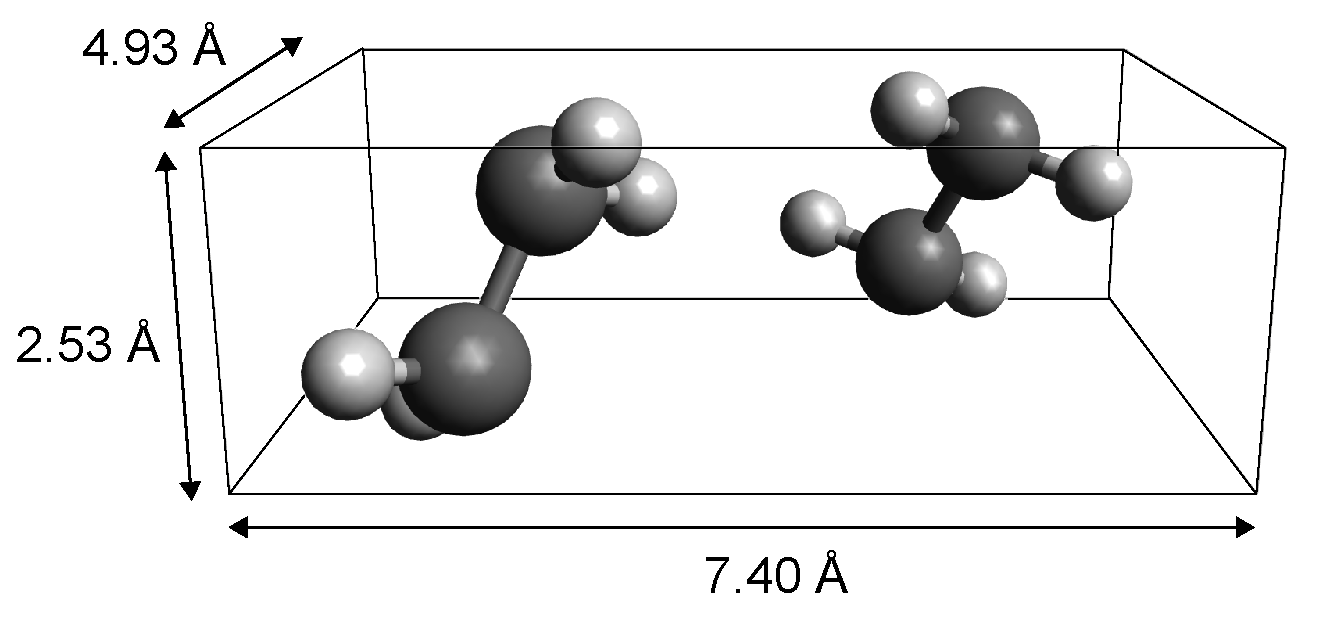
\includegraphics[width=0.4\textwidth]{\figpath/Model1_PE_unitcell_3D.pdf}}

\end{infobox}

\begin{ctqs}
	
	\question Suppose we were to add a single phenyl sidechain to the poly(ethylene) chains, as shown below.

	\vspace{6pt}
	\centerline{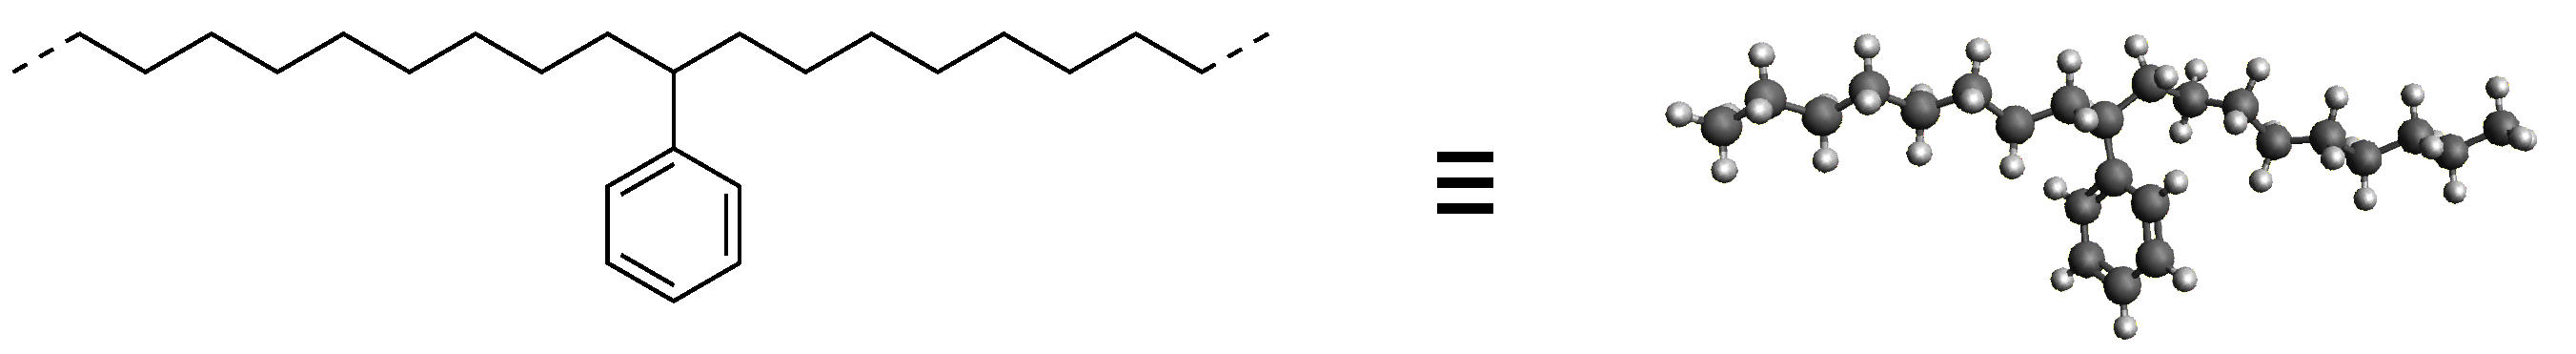
\includegraphics[width=0.8\textwidth]{\figpath/Model1_sidechain.pdf}}	
	
		\begin{enumerate}
		
			\item Would this sidechain be able to ``fit'' easily into the empty spaces in the crystal structure of polyethylene?  Briefly explain why or why not.
	
		\begin{solution}[0.75in]{}
			No, it would not.  It is too bulky.
			
			(Quantitatively, the van der Waals diameter of a phenyl ring is approximately 4-5~\AA.  Even if the first carbon of the ring were right on top of one of the atoms of the polyethylene backbone, the other atoms in the ring would end up on top of the other polymer chain!)
		\end{solution}
			
			\item In the context of your answer to the previous question, do you expect bulky sidechains to make it easier or harder for polymer chains to crystallize?  Explain your group's reasoning in 1-2 complete sentences.
	
		\begin{solution}[1in]{}
			Bulkier side chains should make it more difficult for polymers to pack into regular, repeating crystal structures without significant steric clashes between the sidechains and the other polymer chains (or other sidechains!).  Thus, bulky sidechains should make it more difficult for polymer chains to crystallize.
		\end{solution}
			
		\end{enumerate}
	
	\question Briefly explain how you expect each of the following features of a polymer chain to affect its ability to pack into well-ordered crystal structures:
	
		\begin{enumerate}
		
			\item Stereoregularity (e.g. whether the polymer is isotactic, syndiotactic, or atactic)
	
		\begin{solution}[0.75in]{}
			It should be easiest to pack polymer chains into well-ordered crystals when all of the polymers have the same stereochemistry.  Generally, isotactic polymers are easiest to crystallize and atactic polymers are hardest to crystallize; polypropylene, for example, has degrees of crystallinity on the order of 70-80\%, 50\%, and 0\% for the isotactic, syndiotactic, and atactic stereoisomers, respectively.
		\end{solution}
			
			\item Regioregularity and/or sequence regularity (e.g. how regularly sidechains and functional groups are distributed along the chains)
	
		\begin{solution}[0.75in]{}
			The more regularly the sidechains and functional groups are placed on the polymer chains, the easier it will be for the chains to pack into well-ordered crystals.
			Generally, random copolymers do not crystallize well because the random placement of different sidechains and functional groups inhibits crystal packing.
		\end{solution}
			
			\item Presence of polar functional groups in the polymer backbone that can form hydrogen bonds
	
		\begin{solution}[0.75in]{}
			Strongly polar functional groups in a polymer backbone that can engage in hydrogen bonding, such as those in nylon and other polyamides, can promote arrangement of the polymer chains into well-defined repeating crystal structures.
			
			Note also that in vinyl-type polymers, \textit{small} polar sidechains can also allow crystals to form even if the polymer is atactic; poly(vinyl alcohol), for example, can be semicrystalline.
		\end{solution}
			
		\end{enumerate}
	
\end{ctqs}

\begin{model}[Thermodynamics of Polymer Crystals]
\label{\labelbase:mdl:thermodynamics}
	
	In crystalline polymers, the crystals often form layered structures called \emph{lamellae}, which in turn organize into larger structures such as spherulites, as shown below:
	
	\vspace{6pt}
	\centerline{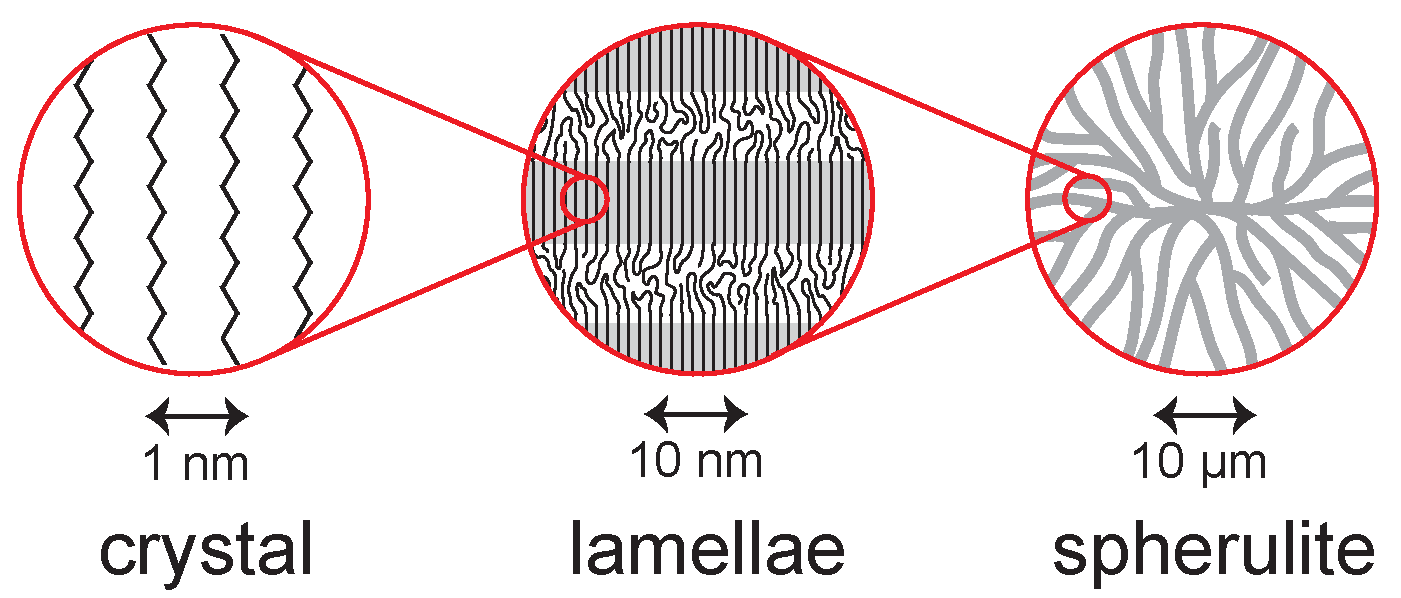
\includegraphics[width=0.8\textwidth]{\figpath/Model2_lengthscales.pdf}}
	
\end{model}

\begin{ctqs}

	\question As shown in the model, does \emph{all} of the polymer in sample form well-ordered crystals?  If not, where are more amorphous/non-crystalline regions found?
	
		\begin{solution}[0.75in]{}
			No, the polymer is not all in well-ordered crystals.  The regions between the layers (lamellae) in the middle image are amorphous/non-crystalline.
		\end{solution}
		
	\question Are the amorphous regions more or less ordered than the crystalline regions?
	
		\begin{solution}[0.5in]{}
			The amorphous regions are less ordered than the crystalline regions (there is more randomness in how the chains are arranged).
		\end{solution}
	
	\question Based on your answer to the previous question, do you expect the entropy of the polymer to increase or decrease as crystalline lamellae melt and become amorphous?  Briefly explain your group's reasoning.
	
		\begin{solution}[0.75in]{}
			The entropy of the polymer should increase as the crystals melt and becomes amorphous, because chains in the amorphous regions are more disordered and there are more ways that the chains can arrange.
		\end{solution}
	
	\question In which region (amorphous or crystalline) do you expect the polymer chains to be able to engage in the most favorable interactions (such as van der Waals interactions) with their neighbors?
	
		\begin{solution}[0.75in]{}
			Interactions such as van der Waals interactions between the chains should be more favorable in the crystalline regions, because the chains effectively have more contact with each other.
		\end{solution}
	
	\question Based on your answer to the previous question, do you expect the enthalpy of the polymer to increase or decrease as crystalline lamellae melt and become amorphous?  Briefly explain your group's reasoning.
	
		\begin{solution}[0.75in]{}
			The enthalpy of the polymer should increase as the crystalline regions melt and become amorphous, because we have to put energy in to break apart favorable interactions.
			
			(Recall that melting is an endothermic process, and for endothermic processes, $\Delta H > 0$.) 
		\end{solution}
		
\end{ctqs}

\begin{infobox}
	The enthalpy change upon melting (i.e. the \emph{enthalpy of fusion}) for a crystal of volume $V$ is
	\begin{equation*}
		\Delta H_f = V\left( H_V^{melt} - H_V^{cryst} \right)
	\end{equation*}
	where $H_V^{melt}$ and $H_V^{cryst}$ are the enthalpies \emph{per unit volume} of the amorphous melt and the crystal, respectively.   The enthalpy of fusion is, similarly,
	\begin{equation*}
		\Delta S_f = V \left( S_V^{melt} - S_V^{cryst} \right)
	\end{equation*} 
\end{infobox}

\begin{ctqs}

	\question Write an expression for the Gibbs free energy of fusion at temperature $T$.
	
		\begin{solution}[0.75in]{}
			\begin{equation*}
				\Delta G_f = \Delta H_f - T\Delta S_f
			\end{equation*}
		\end{solution}
	
	\question The equilibrium melting temperature occurs when $\Delta G_f = 0$.  Find an expression for the equilibrium melting temperature in terms of $H_V^{melt}$, $H_V^{cryst}$, $S_V^{melt}$, and $S_V^{cryst}$. \label{\labelbase:ctq:Tmelt1}
	
		\begin{solution}[1.25in]{}
			\begin{align*}
				0 &= \Delta H_f - T\Delta S_f \\
				T &= \frac{\Delta H_f}{\Delta S_f} = \frac{V\left( H_V^{melt} - H_V^{cryst} \right)}{V \left( S_V^{melt} - S_V^{cryst} \right)} = \frac{\left( H_V^{melt} - H_V^{cryst} \right)}{ \left( S_V^{melt} - S_V^{cryst} \right)}
			\end{align*}
		\end{solution}
	
	\question Based on your answer to the previous question, should the equilibrium melting temperature of a polymer crystal depend on the size or dimensions of the crystalline lamellae?  Explain your group's reasoning in 1-2 complete sentences.
	
		\begin{solution}[1in]{}
			No.  The V's cancelled out, so the equilibrium melting temperature does not depend on the volume of the crystals (or any other parameter related to their size or dimensions).
		\end{solution}
	
\end{ctqs}

\begin{infobox}
	Experimentally, we find that the melting temperatures of semicrystalline polymers \emph{do} depend on the thickness of the crystalline lamellae.  
	The reason turns out to be that the free energy of fusion depends not only on the entropy and enthalpy of the \textit{bulk} crystal, but also on the \textit{surface tension} between the crystal and the surrounding molten or amorphous polymer.
	
	It can be shown (see Exercise \ref{\labelbase:exc:lamellaeTmelt}) that the equilibrium melting temperature of a polymer in which the lamellae have thickness $l$ is given by \label{\labelbase:info:lamellaeTmelt}
		\begin{equation*}
			T_m = \frac{\Delta H^\infty_V}{\Delta S^\infty_V}\left(1-\frac{2\gamma}{l \Delta H^\infty_V}\right)
		\end{equation*}
		where $\Delta H^\infty_V = H^{melt}_V - H^{crystal}_V$, $\Delta S^\infty_V = S^{melt}_V - S^{crystal}_V$,
		and $\gamma$ is the Gibbs free energy per unit area of the crystal/melt interface.
		
\end{infobox}
	
\begin{ctqs}	
	
	\question If $l\to\infty$, what is the melting temperature $T_m^\infty$ in terms of $\Delta H_f^\infty$, $\Delta S_f^\infty$, and any other relevant constants?
	
		\begin{solution}[1in]{}
			When $l\to\infty$,
			\begin{equation*}
				T_m = \frac{\Delta H_V^\infty}{\Delta S_V^\infty}
			\end{equation*}
			(which is the same equation we came up with in CTQ \ref{\labelbase:ctq:Tmelt1}!)
		\end{solution}
			
	\question According to this equation, do finite-thickness lamellae usually have a higher or lower melting temperature than infinite polymer crystals?
	
		\begin{solution}[1in]{}
			Finite-thickness lamellae have lower melting temperatures than infinite polymer crystals (the $-\frac{2\gamma}{l \Delta H^\infty_V}$ term is more negative when $l$ is smaller).
		\end{solution}
	
	\question Explain, in 2-3 complete sentences, how you could determine $T_m^\infty$ from data about the melting temperature of a polymer as a function of lamellar thickness.
	
		\begin{solution}[1.5in]{}
			To determine $T_m^\infty$, you would need to measure the melting temperatures of crystals with different lamellar thicknesses, and then plot the measured melting temperature vs $1/l$.  The y intercept of this plot would be $T_m^\infty$ (and the slope would give information about $\gamma/\Delta H_V^\infty$).
		\end{solution}
 
\end{ctqs}

%\begin{model}[Crystallization Kinetics]
%	\label{\labelbase:mdl:kinetics}
%
%	Most crystals form by nucleation-and-growth processes, as illustrated below:
%	
%\end{model}
%
%\begin{ctqs}
%	
%	\question \dots
%	
%\end{ctqs}

\begin{exercises}

%	\exercise Give a ``predict which of these pairs of polymers will produce the most crystalline structures'' question

	\exercise Based on the unit cell structure shown on page \pageref{\labelbase:info:PEcrystal}, what is the density of crystalline poly(ethylene), in g/m\textsuperscript{3}?
	
		\begin{solution}{}
		
		The unit cell shown on page \pageref{\labelbase:info:PEcrystal} contains 4 carbon atoms and 8 hydrogen atoms, for a total mass of $4(12.01\text{ amu}) + 8(1.00\text{ amu}) = 56.04\text{ amu}$.
		
		The volume of the unit cell is $(4.93~\AA)(2.53~\AA)(7.40~\AA) = 92.30~\AA^3$.
		
		The density is thus
		\begin{align*}
			\rho = \frac{\left(56.04\text{ amu}\right)\left(\frac{1.66\times 10^{-27}\text{ kg}}{1\text{ amu}}\right)}{(92.30~\AA^3)\left(\frac{10^{-10}\text{ m}}{1~\AA}\right)^3} = 1007~\text{kg/m}^3
		\end{align*}
		or approximately 1~g/cm\textsuperscript{3}.
		
		\end{solution}
	
	\exercise In Model \ref{\labelbase:mdl:thermodynamics}, you learned how changes in the lamellar thickness impact the melting temperature of polymer crystals. A similar analysis can be used to determine how changes in polymer molecular weight impact melting temperature.  In particular, one finds that
		\begin{equation*}
			\Delta H_f\left(\frac{1}{T_m} - \frac{1}{T_m^\infty}\right) = \frac{2 R M_0}{M_n}
		\end{equation*}
		
		According to this equation, does increasing the molecular weight of a polymer generally increase or decrease its melting temperature?  Explain your reasoning in 1-2 complete sentences.
	
		\begin{solution}{}
		
		The equation given in this question can be rearranged to the form
		\begin{equation*}
			\frac{1}{T_m} = \frac{2RM_0}{M_n\Delta H_f} + \frac{1}{T_m^\infty}
		\end{equation*}
		
		As the molecular weight of the polymer ($M_n$) is increased, the magnitude of the 	$\frac{2RM_0}{M_n\Delta H_f}$ term decreases.  This in turn decreases the value of $1/T_m$, which corresponds to increasing $T_m$.  Thus, as the molecular weight of a polymer increases, its melting temperature also generally increases.	
		
		\end{solution}
		
	\exercise Derive the expression for $T_m$ given on page \pageref{\labelbase:info:lamellaeTmelt} by considering the following segment of a crystalline lamella: \label{\labelbase:exc:lamellaeTmelt}
	
		\centerline{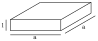
\includegraphics[width=0.4\textwidth]{\figpath/Exc_xtaldimensions.pdf}}
		
		For the purposes of this problem, we will assume that this crystalline segment is in contact with the amorphous melt on all sides.
	
		\begin{enumerate}
			
			\item Determine the volume and surface area of this segment in terms of the given dimensions.
			
				\begin{solution}{}
					The volume is $V=a^2 l$
					
					The surface area is $A = 2a^2 + 4 al$ (remember to include the faces of the solid that we can't see!).
				\end{solution}
			
			\item Assuming the volumetric enthalpy and entropy of the crystal are $H_V^{cryst}$ and $S_V^{cryst}$, and the Gibbs free energy per unit area of the melt/crystal interface is $\gamma$, determine the total free energy of this crystalline segment at temperature $T$.
			
				\begin{solution}{}
					\begin{align*}
						G^{cryst} &= V\,H_V^{cryst} -T V\, S_V^{cryst} + \gamma A \\
							&= a^2 l\,H_V^{cryst} -T a^2 l\, S_V^{cryst} + \gamma (2a^2 + 4 al)
					\end{align*}
				\end{solution}
			
			\item Assuming the volumetric enthalpy and entropy of the melt are $H_V^{melt}$ and $S_V^{melt}$, determine the total free energy of the polymer in this segment after it has melted.  You may assume that the volume does not change upon melting.
			
				\begin{solution}{}
					\begin{align*}
						G^{melt} &= V\,H_V^{melt} -T V\, S_V^{melt} \\
							&= a^2 l\,H_V^{melt} -T a^2 l\, S_V^{melt}
					\end{align*}
					(Note that there is no contribution from $\gamma$ because there is no remaining crystal/melt interface after melting.)
				\end{solution}
				
			\item Combine your answers to the previous two parts to obtain an expression for the free energy of fusion (free energy change during melting), and determine the temperature at which equilibrium will occur.
			
				\begin{solution}{}
					\begin{align*}
						\Delta G_f &= G^{melt} - G^{cryst} \\
						&= (a^2 l\,H_V^{melt} -T a^2 l\, S_V^{melt}) - (a^2 l\,H_V^{cryst} -T a^2 l\, S_V^{cryst} + \gamma (2a^2 + 4 al))
					\end{align*}
					Equilibrium is reached when $\Delta G_f = 0$, or
					\begin{align*}
						a^2 l\,H_V^{melt} -T a^2 l\, S_V^{melt} = a^2 l\,H_V^{cryst} -T a^2 l\, S_V^{cryst} + \gamma (2a^2 + 4 al)
					\end{align*}
					Solving for $T$ and simplifying, we obtain
					\begin{align*}
						T (a^2 l\, S_V^{cryst} - a^2 l\, S_V^{melt}) &= a^2 l\,H_V^{cryst} + \gamma (2a^2 + 4 al) - a^2 l\,H_V^{melt}\\
						T &= \frac{a^2 l\,H_V^{cryst} + \gamma (2a^2 + 4 al) - a^2 l\,H_V^{melt}}{a^2 l\, S_V^{cryst} - a^2 l\, S_V^{melt}}\\
						 &= \frac{H_V^{cryst} + \gamma (\frac{2}{l} + \frac{4}{a}) - H_V^{melt}}{S_V^{cryst} - S_V^{melt}} \\
						 &= \frac{\Delta H_V^\infty - \gamma\left(\frac{2}{l} + \frac{4}{a}\right)}{\Delta S_V^\infty} \\
						 &= \frac{\Delta H_V^\infty}{\Delta S_V^\infty}\left(1-\frac{\gamma}{\Delta H_V^\infty}\left(\frac{2}{l} + \frac{4}{a}\right)\right)
					\end{align*}
				\end{solution}
			
			\item In the limit that $a \gg l$, the term that goes as $\frac{1}{a}$ can be ignored because it is much smaller than the term that goes as $\frac{1}{l}$.  Verify that dropping this term yields the expression given on page \pageref{\labelbase:info:lamellaeTmelt}, as desired.
			
				\begin{solution}{}
					Dropping the $4/a$ term yields
					\begin{align*}
						T &= \frac{\Delta H_V^\infty}{\Delta S_V^\infty}\left(1-\frac{\gamma}{\Delta H_V^\infty}\frac{2}{l}\right) \\
						 &= \frac{\Delta H_V^\infty}{\Delta S_V^\infty}\left(1-\frac{2\gamma}{l\Delta H_V^\infty}\right)
					\end{align*}
					as desired.
				\end{solution}
			
		\end{enumerate}
	
\end{exercises}


%\begin{problems}
%
%	\problem First exercise
%	\problem Second exercise
%	
%\end{problems}


	
\end{activity}